% !TEX program = xelatex

\documentclass{VUMIFPSkursinis}
\usepackage{algorithmicx}
\usepackage{algorithm}
\usepackage{algpseudocode}
\usepackage{amsfonts}
\usepackage{amsmath}
\usepackage{bm}
\usepackage{caption}
\usepackage{color}
\usepackage{float}
\usepackage{graphicx}
\usepackage{listings}
\usepackage{float}
\usepackage{subfig}
\usepackage{wrapfig}
\usepackage[hidelinks]{hyperref}
\usepackage{todonotes}
\usepackage{lineno}
\usepackage{pdflscape}


% Titulinio aprašas
\university{Vilniaus universitetas}
\faculty{Matematikos ir informatikos fakultetas}
\department{}
\papertype{Programų sistemų inžinerijos modeliai ir metodai laboratorinis darbas 2}
\title{Requirements modeling}
\titleineng{Reikalavimų modeliavimas}
\status{1 course students}
\author{Matas Savickis}
\secondauthor{Vytautas Krivickas}
\thirdauthor{Šarūnas Kazimieras Buteikis}


\supervisor{Audronė Lupeikienė, M. Darbuot., Dr}
\date{Vilnius – \the\year}

% Nustatymai
% \setmainfont{Palemonas}   % Pakeisti teksto šriftą į Palemonas (turi būti įdiegtas sistemoje)
\bibliography{bibliografija}

\begin{document}
\selectlanguage{english}
\maketitle

\tableofcontents

\section{NFR type catalogue}

\begin{figure}[htbp]
	\center
	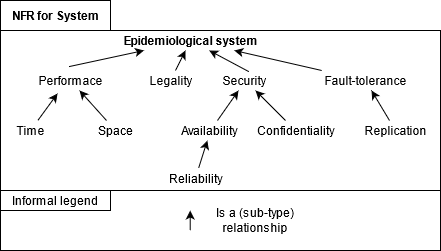
\includegraphics[scale=0.9]{img/1}
	\caption{NFR diagram} % Antraštė įterpiama po paveikslėlio
	\label{img:kurimoProcesas}
\end{figure}

	\begin{itemize}
		%\item{\textbf{Virus registration time} - to ensure quick response time system must provide quick process of registering new cases. }
		%\item{\textbf{Patient notification time} - it is important to prevent spread of virus by hastily notifying and isolating contagious patients.}
		%\item{\textbf{Holding medical records} - to ensure that the spread of the epidemic is contained and monitored, all necessary medical records related to the epidemic must be accessed via the system. }
		%\item{\textbf{Holding foreign countries data} - to check which countries are infected and are spreading the virus, the epidemiological system has to keep up-to-date epidemiological information about them.}
		\item{\textbf{Time} - System is monitoring the epidemic therefore its processes or workflows have to be efficient time-wise.}
		\item{\textbf{Space} - since the system will contain lots of different data (e.g. person's geographical coordinates), data must be stored efficiently.}		
		\item{\textbf{Reliability} - Tracking the state of the epidemic must be ensured 24/7 to not miss any crucial data or trends.}
		\item{\textbf{Confidentiality} - the epidemiological system must treat sensitive personal information (e.g. received medical records) to ensure systems credibility.}
		\item {\textbf{Legality} - due to the fact the epidemiological system will deal with sensitive information, data handling must comply with LT and EU data laws as well as GDPR.}
		\item{\textbf{Replication} - non-sensitive data must have duplicate records stored to increase the system's fault-tolerance.}
	\end{itemize}

	\begin{landscape}
\section{Modelling of the non-functional requirements}
	\subsection{Self-isolation}
		\begin{figure}[H]
			\center
			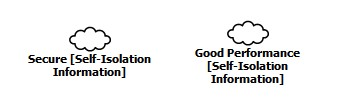
\includegraphics[scale=0.9]{StarUML/Self-Isolation-1}
			\caption{Self Isolation - Initial Software Dependency Graph} % Antraštė įterpiama po paveikslėlio
			\label{img:kurimoProcesas}
		\end{figure}
		\begin{figure}[H]
			\center
			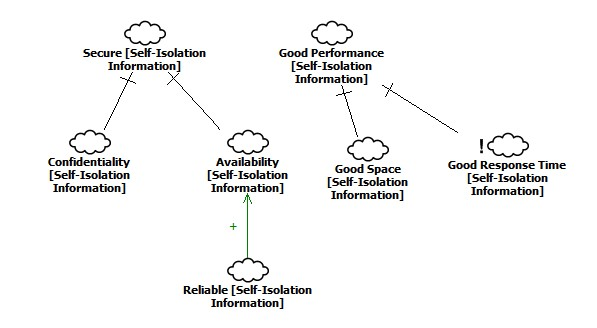
\includegraphics[scale=0.5]{StarUML/Self-Isolation-2}
			\caption{Self Isolation - Decomposing NFRs} % Antraštė įterpiama po paveikslėlio
			\label{img:kurimoProcesas}
		\end{figure}
		

	\subsection{Infected patients}
		\begin{figure}[H]
			\center
			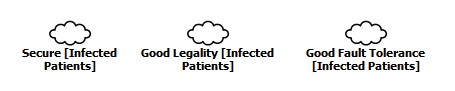
\includegraphics[scale=0.9]{StarUML/Infected-Patients-1}
			\caption{Infected Patients - Initial Software Dependency Graph} % Antraštė įterpiama po paveikslėlio
			\label{img:kurimoProcesas}
		\end{figure}
		\begin{figure}[H]
			\center
			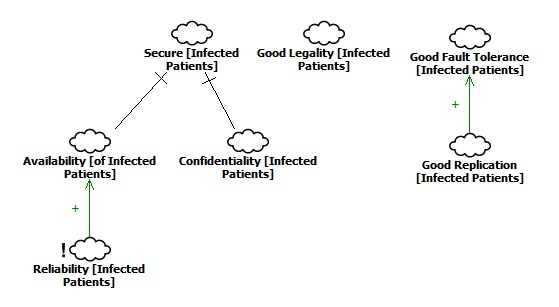
\includegraphics[scale=0.9]{StarUML/Infected-Patients-2}
			\caption{Infected Patients - Decomposing NFRs} % Antraštė įterpiama po paveikslėlio
			\label{img:kurimoProcesas}
		\end{figure}



	\subsection{Dangerouse countries}
		\begin{figure}[H]
			\center
			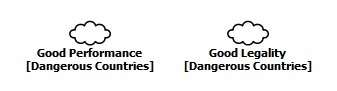
\includegraphics[scale=0.9]{StarUML/Dangerous-Countries-1}
			\caption{Dangerous Countries - Initial Software Dependency Graph} % Antraštė įterpiama po paveikslėlio
			\label{img:kurimoProcesas}
		\end{figure}
		\begin{figure}[H]
			\center
			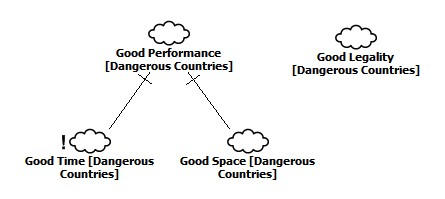
\includegraphics[scale=0.9]{StarUML/Dangerous-Countries-2}
			\caption{Dangerous Countries - Decomposing NFRs} % Antraštė įterpiama po paveikslėlio
			\label{img:kurimoProcesas}
		\end{figure}	

\section{Identifying and modelling of possible operationalizations for NFR}
	\subsection{Self-isolation}
			\begin{figure}[H]
				\center
				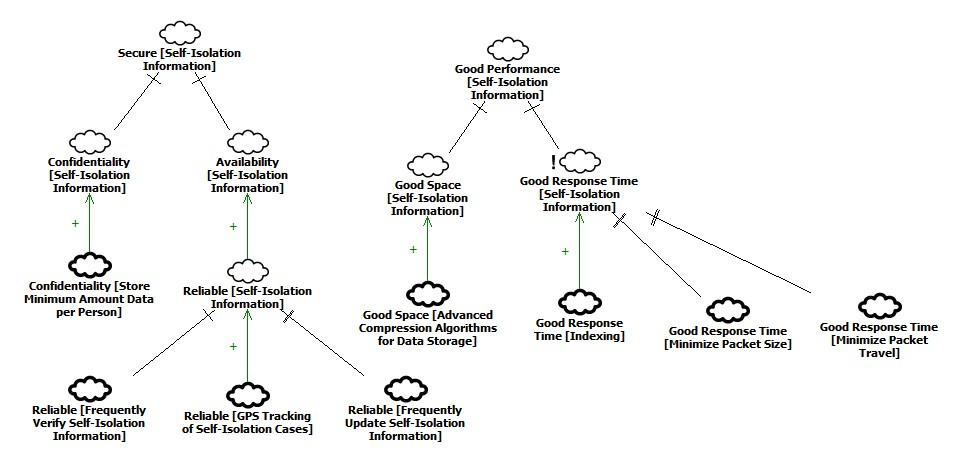
\includegraphics[scale=0.6]{StarUML/Self-Isolation-3}
				\caption{Self Isolation - Possible Operationalizations} % Antraštė įterpiama po paveikslėlio
				\label{img:kurimoProcesas}
			\end{figure}
		
	\subsection{Infected patients}
		\begin{figure}[H]
			\center
			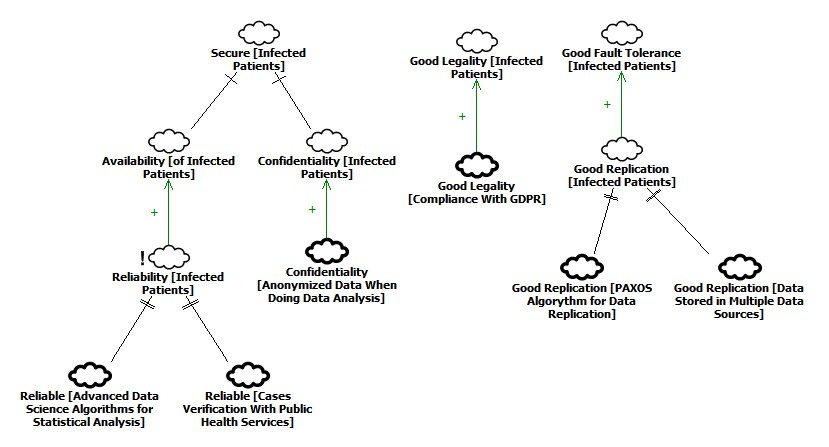
\includegraphics[scale=0.6]{StarUML/Infected-Patients-3}
			\caption{Infected patients - Possible Operationalizations} % Antraštė įterpiama po paveikslėlio
			\label{img:kurimoProcesas}
		\end{figure}

	\subsection{Dangerouse countries}
		\begin{figure}[H]
			\center
			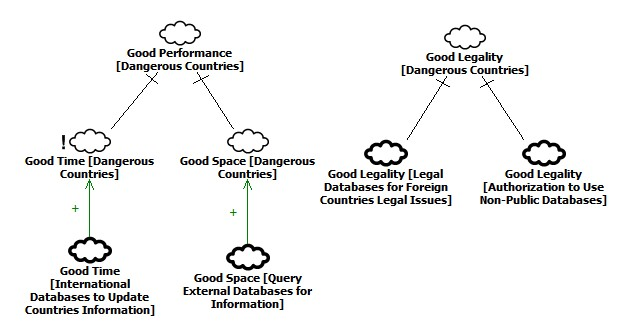
\includegraphics[scale=0.6]{StarUML/Dangerous-Countries-3}
			\caption{Dangerous Countries - Possible Operationalizations} % Antraštė įterpiama po paveikslėlio
			\label{img:kurimoProcesas}
		\end{figure}	

\section{Detecting and Modelling of Implicit Interdependencies Among NFR}
	\begin{figure}[H]
		\center
		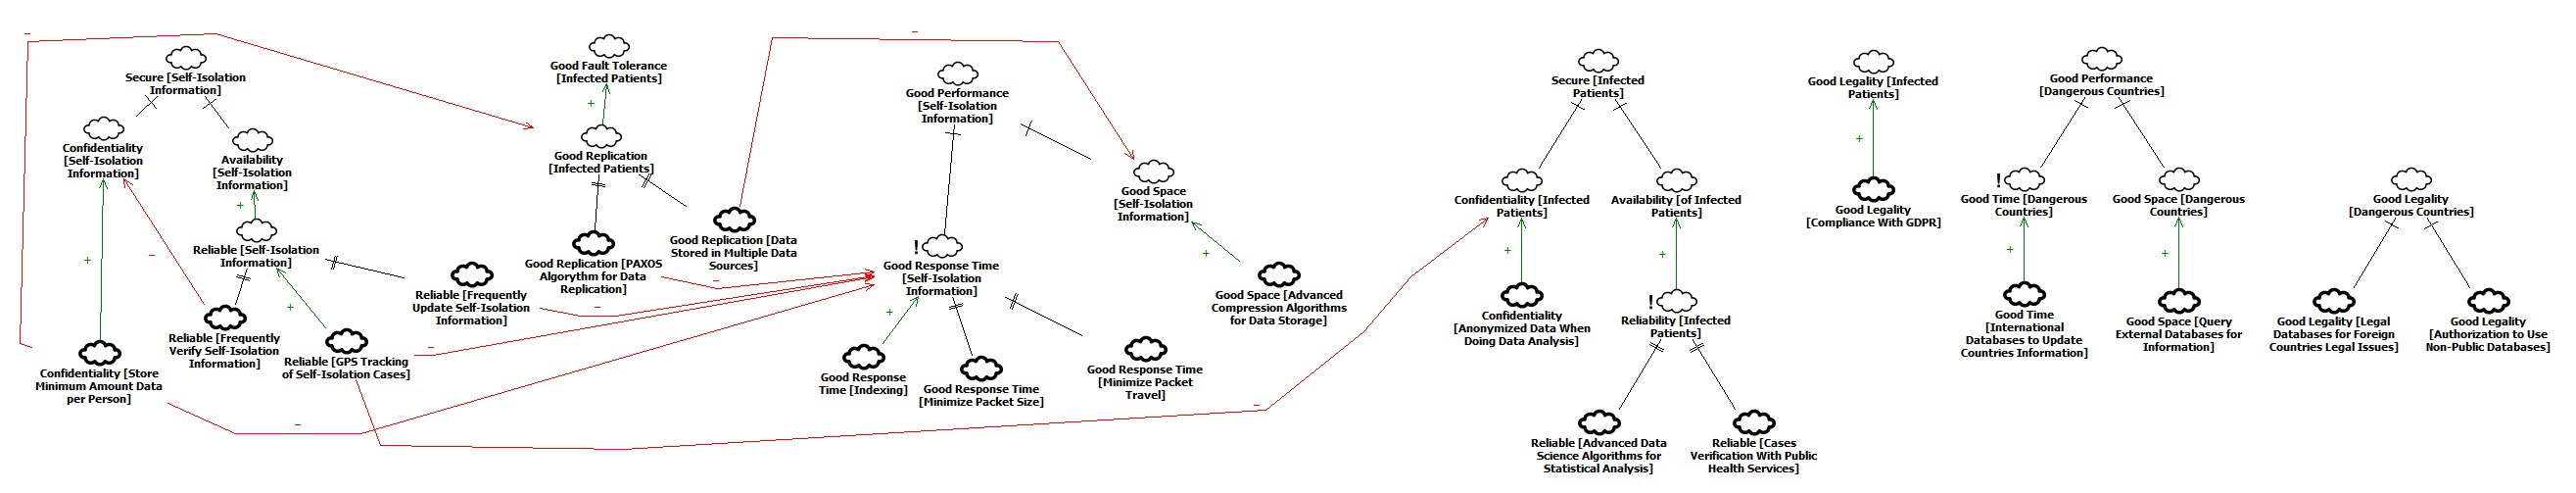
\includegraphics[scale=0.3]{StarUML/Implicit-InterDependencies}
		\caption{Implicit interdependencies among NFRs} % Antraštė įterpiama po paveikslėlio
		\label{img:kurimoProcesas}
	\end{figure}
\section{Making decisions}
\subsection{Chosen Operationalizations and SoftGoals}
	\begin{figure}[H]
		\center
		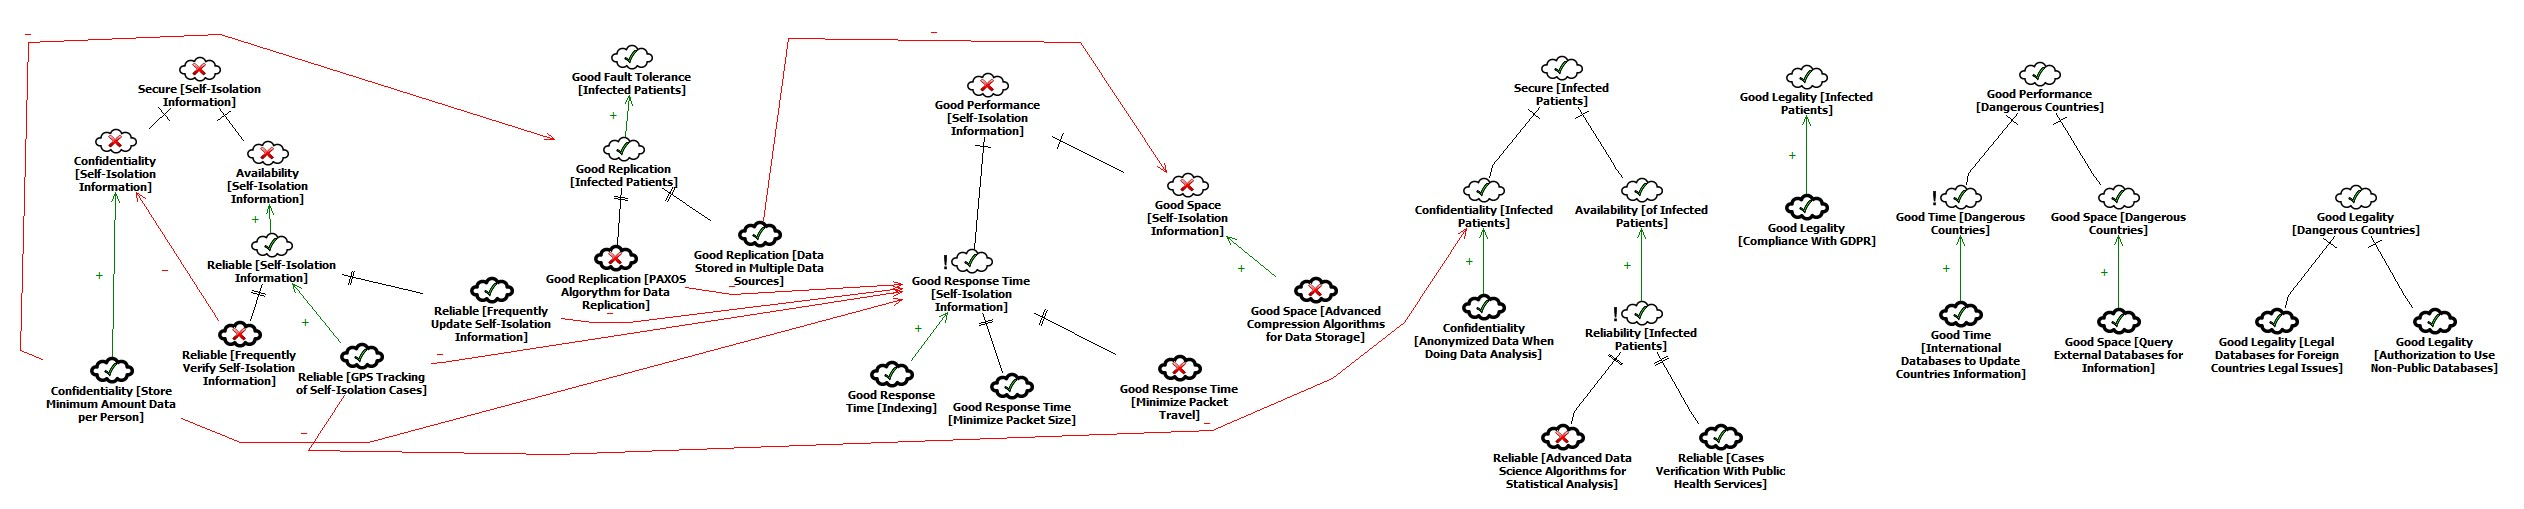
\includegraphics[scale=0.3]{StarUML/Chosen-Operationalizations}
		\caption{Chosen Operationalizations among NFRs} % Antraštė įterpiama po paveikslėlio
		\label{img:kurimoProcesas}
	\end{figure}
\end{landscape}
\subsection{Decision Explanation}
	\subsubsection{Negative impact}
		\begin{itemize}
			\item{Frequantly verify self-isolation information harms confidentiality because increasing amounts of data are processed with an increased chance for data interception.}
			\item{Store minimum amount of data about a person hurts good response time because querying small unstructured data takes longer.}
			\item{Store minimum amount of data about a person harms good replication because replication requires a lot of data to work properly.}
			\item{GPS tracking of self-isolation cases harms confidentiality because in case of data breach intruders might gain the ability to know  a person's location.}
			\item{GPS tracking of self-isolation cases hurts good response time because updating GPS information takes a long time.}
			\item{Frequently update self-isolation information harms response time because it takes computer resources to do the update.}
			\item{Use PAXOS algorithm for replication harms response time because this algorithm takes a lot of computational resources to complete. Which impacts response time.}
			\item{Data stored in multiple data sources hurts good space because it takes a lot of physical computer space to store in multiple sources.}
		\end{itemize}
	\subsubsection{Rejected operationalization}
		\begin{itemize}
			\item{Frequantly verify self-isolation information - verification usually can be a complex process also it heavily impacts confidentiality, that's why we decided to reject.}
			\item{Advanced protocol to minimize packet travel - lack of competency in the team to implement such protocols.}
			\item{Use advanced compression algorithms for data storage - lack of competency in the team to implement such algorithms.}
			\item{Apply advanced data science algorithms for statistical analysis - lack of competency in the team to implement such algorithms.}
			\item{Use PAXOS algorithm for replication - lack of competency in the team to implement such protocols.}
		\end{itemize}
\subsection{Conclusions}
 Using NFR we successfully selected, decomposed, and chose operationalized soft goals to be completed in our project.
Analysis was very useful and applicable in real-life scenarios in the industry.
\section{Strategic Dependency Model}
\begin{figure}[H]
    \center
    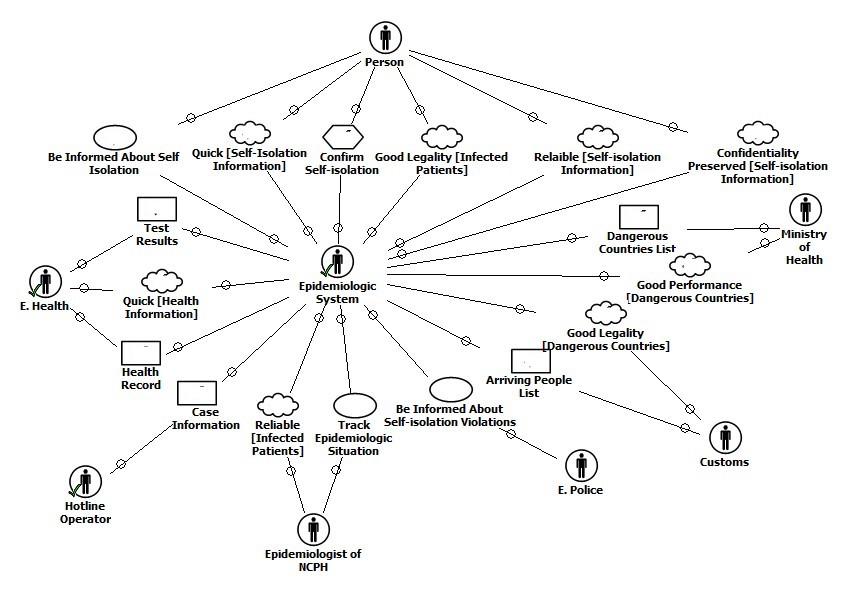
\includegraphics[scale=0.5]{StarUML/Strategic_Dependency.jpg}
    \caption{Strategic Dependency Model} % Antraštė įterpiama po paveikslėlio
    \label{img:strategicDep}
\end{figure}
\section{Strategic Rationale Model}
\begin{figure}[H]
    \center
    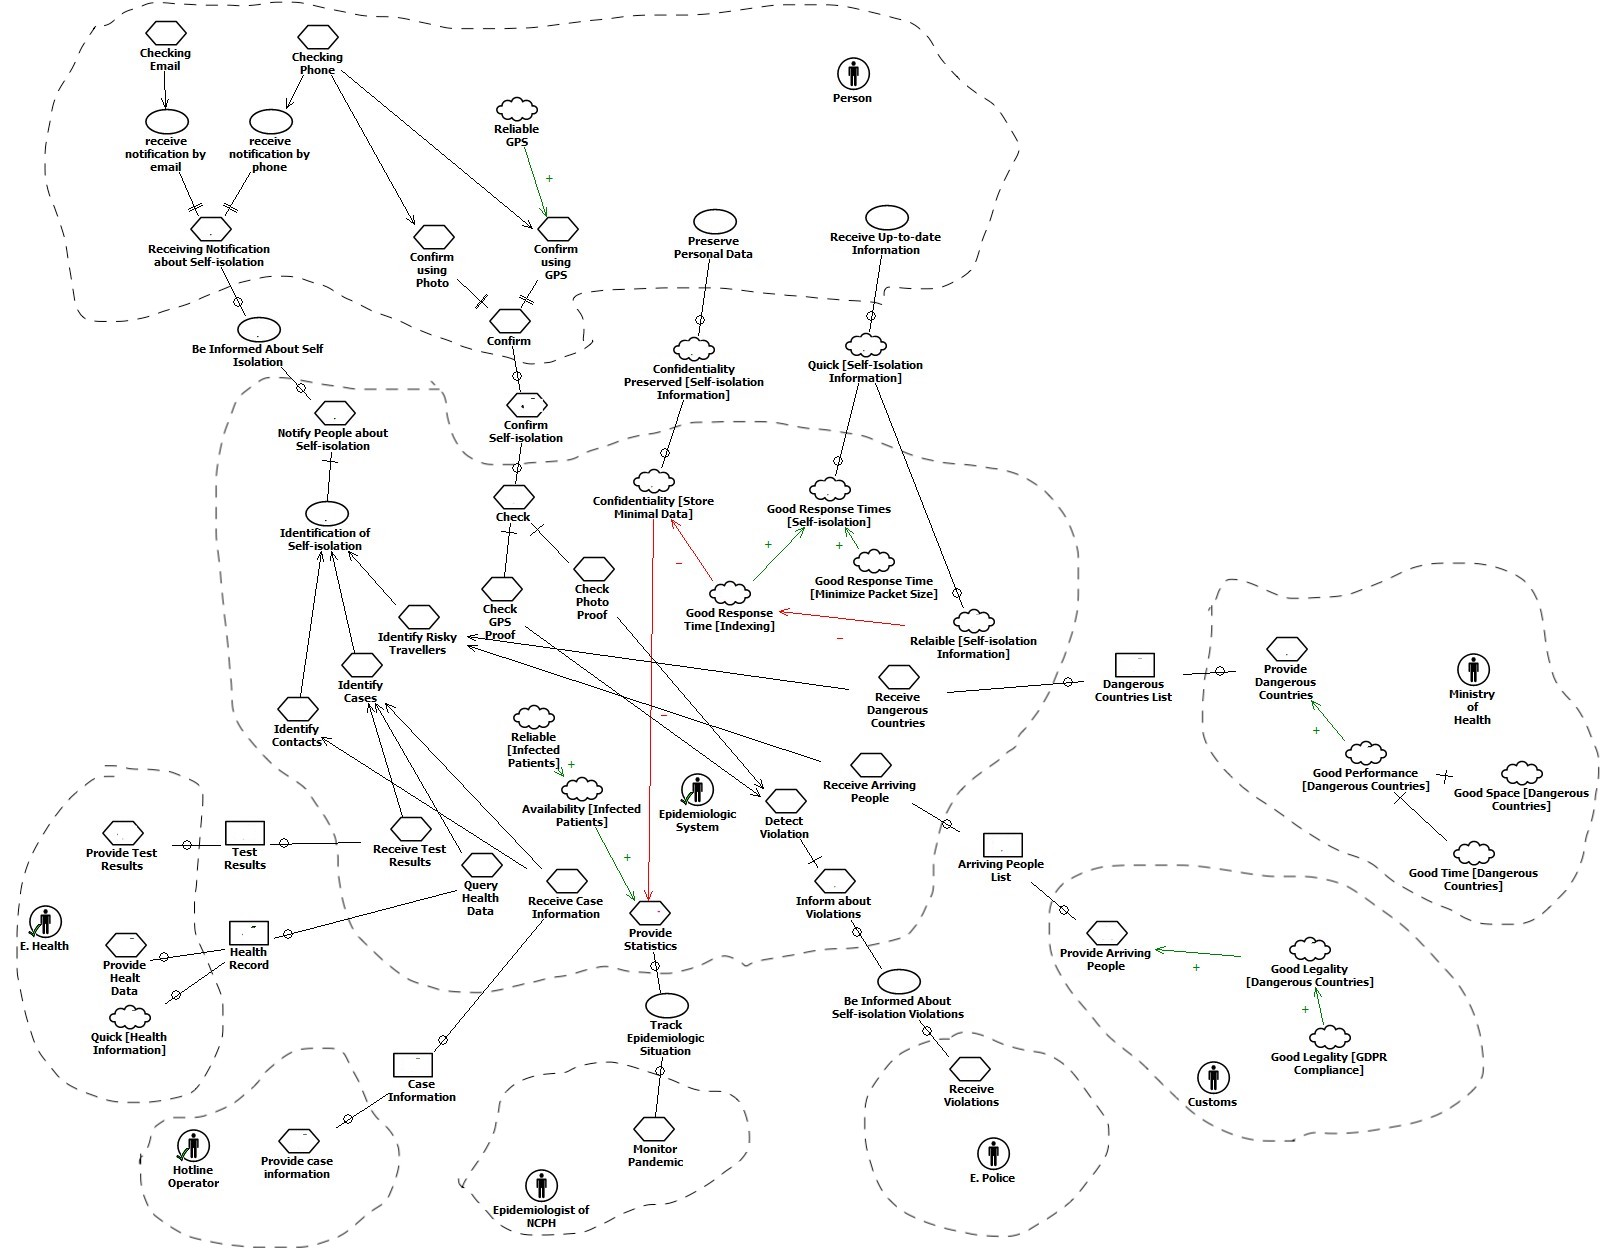
\includegraphics[scale=0.3]{StarUML/Strategic_Rationale.jpg}
    \caption{Strategic Rationale Model} % Antraštė įterpiama po paveikslėlio
    \label{img:strategicRationale}
\end{figure}
\section{Conclusions about an dependency}
	
\sectionnonum{Conclusions}

Inconsistencies between non functional requirements have been identified and eliminated by selecting appropriate operalizations. For achieving 
secure self-isolation information, it is recommended to store minimunm amount of data per person and use reliable GPS tracking. To achieve good fault tolerance for 
statistics (infected patients), it is recommended to store data in multiple data centers. To achieve good performance (self-isolation information), it is recommended
to use indexing and minimize packet size. To ensure security of infected patients statistics, it is recommended to anonymyze data when conducting 
data analysis and verify cases with public health services. To achieve good legality, it is recommended to ensure GDPR compliance, and collect required permits. Finally, 
to ensure good performance of dangerous countries retrieval, it is recommended to query external databases for information and use international databases
to update countries information.

\end{document}
